% This LaTeX was auto-generated from MATLAB code.
% To make changes, update the MATLAB code and export to LaTeX again.

\documentclass{article}

\usepackage[utf8]{inputenc}
\usepackage[T1]{fontenc}
\usepackage{lmodern}
\usepackage{graphicx}
\usepackage{color}
\usepackage{hyperref}
\usepackage{amsmath}
\usepackage{amsfonts}
\usepackage{epstopdf}
\usepackage[table]{xcolor}
\usepackage{matlab}

\sloppy
\epstopdfsetup{outdir=./}
\graphicspath{ {./comparecosts_images/} }

\begin{document}

\matlabtitle{Compare Gasoline Cost}

\begin{par}
\begin{flushleft}
Compares the cost of gasoline in Australia with other countries. 
\end{flushleft}
\end{par}

\begin{par}
\begin{flushleft}
The true cost (in terms of hours of labor) of a liter of gasoline is calculated from raw price data and average hourly wages. The cost in Australia is compared to Canada, Germany, and Mexico. Statistics are calculated for the difference bewteen Australia and Canada.
\end{flushleft}
\end{par}


\matlabheading{Load gas price data from file}

\begin{par}
\begin{flushleft}
Replace the missing Australian price in 1990 with the price in 1991.
\end{flushleft}
\end{par}

\begin{matlabcode}
load gCosts
Australia(1) = Australia(2);
\end{matlabcode}


\matlabheading{Plot the gas prices for all four countries.}

\begin{matlabcode}
plot(Year,Australia,".-")
hold on
plot(Year,Canada,".--")
plot(Year,Germany,".--")
plot(Year,Mexico,".--")
hold off
% Add annotations
legend(country,"Location","northwest")
title("Annual gasoline prices")
xlabel("Year")
ylabel("Price [US$/gallon]")
\end{matlabcode}
\begin{center}
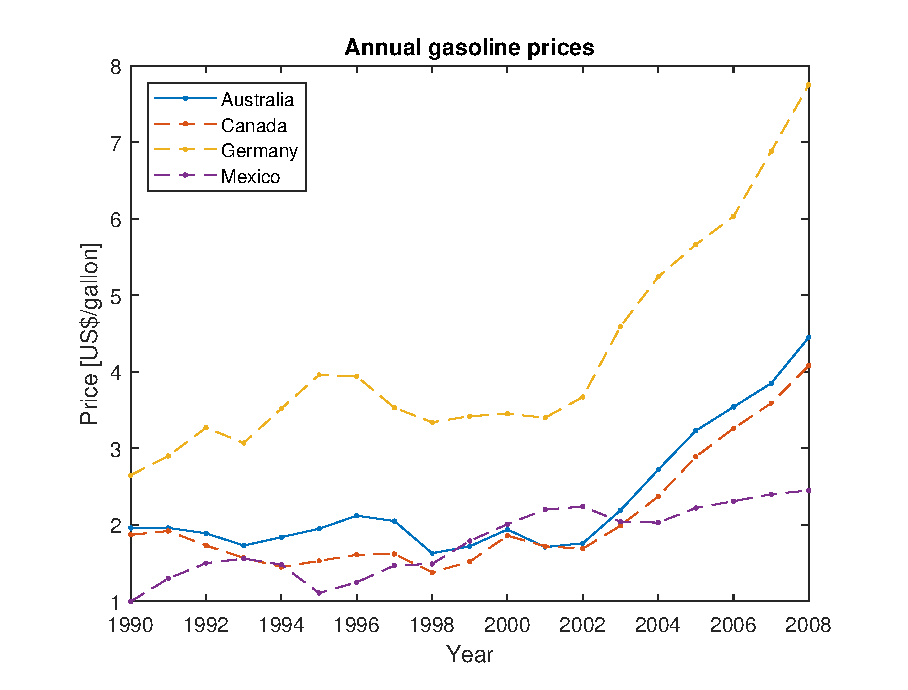
\includegraphics[width=\maxwidth{56.196688409433015em}]{figure_0.eps}
\end{center}


\matlabheading{Convert the prices to costs.}

\begin{par}
\begin{flushleft}
The units for cost are work hours (based on average income) per liter.
\end{flushleft}
\end{par}

\begin{par}
$$\frac{hour}{L}=\frac{gal}{L}\times \frac{USD}{gal}\div \frac{USD}{hr}$$
\end{par}

\begin{matlabcode}
gal2lit = 0.2642;
AustraliaHpL = gal2lit*Australia/hourlyAus;
CanadaHpL = gal2lit*Canada/hourlyCan;
GermanyHpL = gal2lit*Germany/hourlyGer;
MexicoHpL = gal2lit*Mexico/hourlyMex;
\end{matlabcode}

\begin{par}
\begin{flushleft}
Plot the costs.
\end{flushleft}
\end{par}

\begin{matlabcode}
plot(Year,AustraliaHpL,".--")
hold on
plot(Year,CanadaHpL,".--")
plot(Year,GermanyHpL,".--")
plot(Year,MexicoHpL,".--")
hold off
% Add annotations
title("Annual gasoline costs")
legend(country,"Location","NorthWest")
xlabel("Year")
ylabel("Cost [Work hours/L]")
\end{matlabcode}
\begin{center}
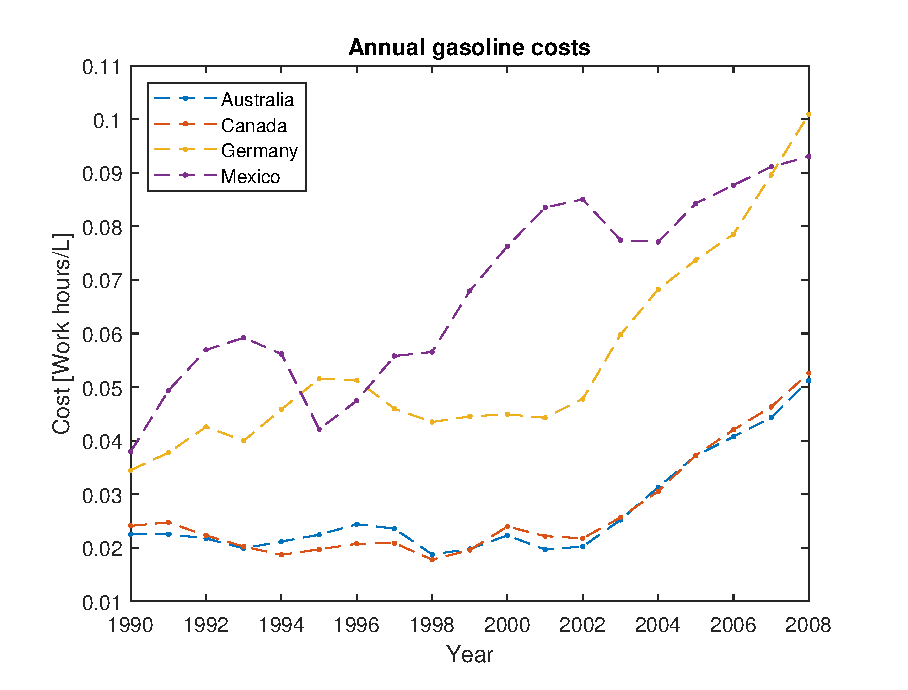
\includegraphics[width=\maxwidth{56.196688409433015em}]{figure_1.eps}
\end{center}


\matlabheading{Calculate the difference between Australian and Canadian cost.}

\begin{matlabcode}
AuCaDiff = CanadaHpL- AustraliaHpL;

% Plot the result
bar(Year,AuCaDiff)
xlabel("Year")
ylabel("Difference in cost [Work hours/L]")
title("Comparison of cost: Canada - Australia")
xlim([1989 2009])
\end{matlabcode}
\begin{center}
\includegraphics[width=\maxwidth{56.196688409433015em}]{figure_2.eps}
\end{center}


\matlabheading{Calculate statistics on the difference.}

\begin{par}
\begin{flushleft}
What was the average difference in cost between Australia and Canada?
\end{flushleft}
\end{par}

\begin{matlabcode}
avgDiff = mean(AuCaDiff)
\end{matlabcode}
\begin{matlaboutput}
avgDiff = 1.0320e-04
\end{matlaboutput}

\begin{par}
\begin{flushleft}
Find the absolute value of the difference. When did the greatest cost difference occur?
\end{flushleft}
\end{par}

\begin{matlabcode}
absDiff = abs(AuCaDiff);
[biggestDiff,idx] = max(absDiff);
Year(idx)
\end{matlabcode}
\begin{matlaboutput}
ans = 1996
\end{matlaboutput}


\matlabheading{Plot the Australian and Canadian costs against each other.}

\begin{matlabcode}
scatter(AustraliaHpL,CanadaHpL,20,Year,"Filled")
xlim([0 0.06])
% Add 45 degree line.
AuLimits = xlim;
hold on
plot(AuLimits,AuLimits,"r")
hold off
% Add annotations.
xlabel("Australian cost [hrs/L]")
ylabel("Canadian cost [hrs/L]")
\end{matlabcode}
\begin{center}
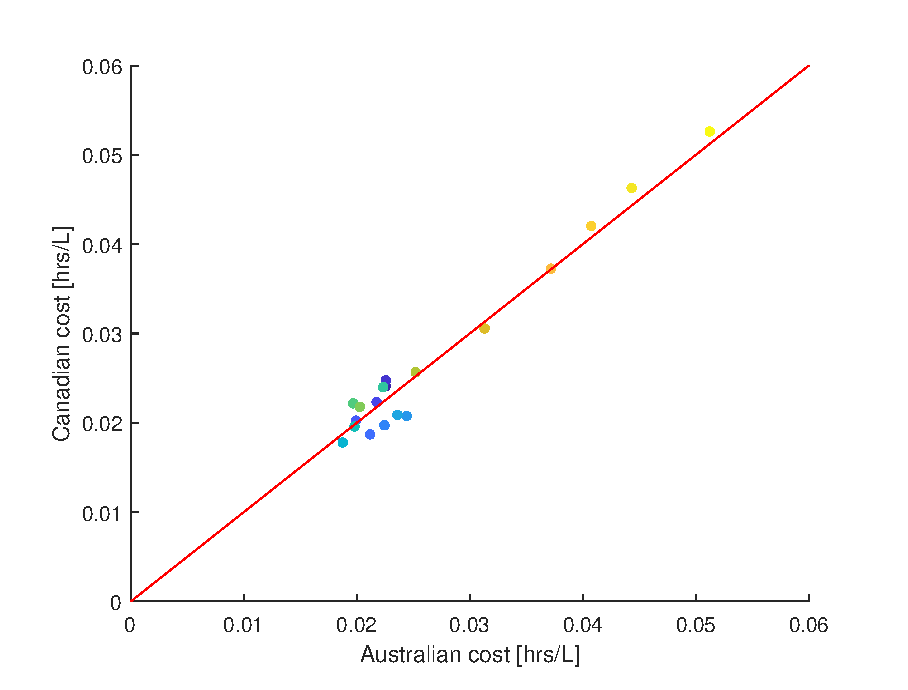
\includegraphics[width=\maxwidth{56.196688409433015em}]{figure_3.eps}
\end{center}

\end{document}
